\documentclass{hitec}
\usepackage[utf8] {inputenc}
\renewcommand{\baselinestretch}{1}
\title{VIV1 Hexacopter Drone Manufacturing Documentation}
\author{Jonas Cronholm}
\date{December 2021}
\usepackage{graphicx}
\graphicspath{images}
\usepackage{animate}
\usepackage{caption}
\usepackage{subcaption}

\begin{document}
	\pagenumbering{Roman}
	\maketitle
	\pagebreak
	\tableofcontents
	\pagebreak
	\section{Preamble}
	\subsection{Document Structure and Introduction}
	This document will begin with a brief introduction to why and how I created this product. Then, I will compare the cost, weight and overall features of my drone to other ones (within a certain comparable range). 
	I will also go over the complete design process in Fusion 360 (there will be illustrations), and also share my mindset while working on a product like this one. This section will also include the software design process.
	Finally, I will include a construction guide with information on how to print, cut and assemble the drone. And a complete guide and documentation concerning the firmware of the drone. \newline  
	\subsection{Description}
	The VIV1 (Roman VI, Version 1), is a Hexacopter designed around the Arduino Mega 2560 platform. The Hexacopter (or drone as I will refer to it as from now on), was an idea born completely out of pure chance. This is due to the fact that I randomly came across parts to a quadrocopter (that had eight brushless motors) which led me to become obsessed with this new project. I sat down and designed a prototype in Fusion 360, which took me about 2.5 hours in total. (see anim. 1)
	\pagebreak
	
	\subsection{Parts List}
	The following table will show all the parts that I used in the construction of this drone.
	\begin{figure}[h]
		\centering
		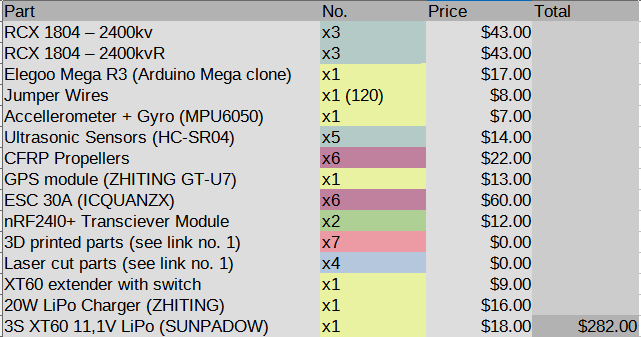
\includegraphics[width=\linewidth]{parts}
		\caption{Parts List}
		\label{fig:pl}
	\end{figure}
	\subsection{Comparison}
	The price of drones can span between hundreds and thousands of dollars, so I chose some select hexacopter DIY kits and some pre-assembled drones to compare the VIV1 to. (fig. 2, red is worse)
		\begin{figure}[h]
		\centering
		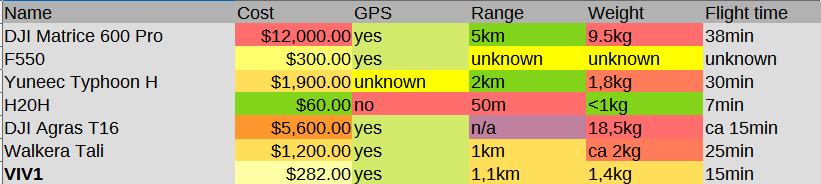
\includegraphics[width=\linewidth]{comp}
		\caption{Comparison Table}
		\label{fig:ct}
	\end{figure}
	\subsection{Conclusion}
	\pagebreak
	\section{Design Process (Hardware)}
	\subsection{Introduction}
	In this chapter I will go over how I designed the first prototype of the VIV1 drone. I will share my design theory, some illustrations of the product (generated by a Fusion 360 script), why I used the materials that I used and some thoughts about the final result.
	\subsection{Design Theory}
	So first, Design theory.\newline
	Rather than having a very fixed idea on how I wanted the drone to look, I simply let my mind create without any limitations regarding weight, size or simplicity. This, of course was maybe not the best idea as it made me skip some rather important parts of the design process that would have to be taken into consideration later.\newline
	I begun with designing the arms (see fig. 3). I decided to take inspiration from the DJI F550, and begun working on a draft. \newline
	\begin{figure}[h]
		\centering
		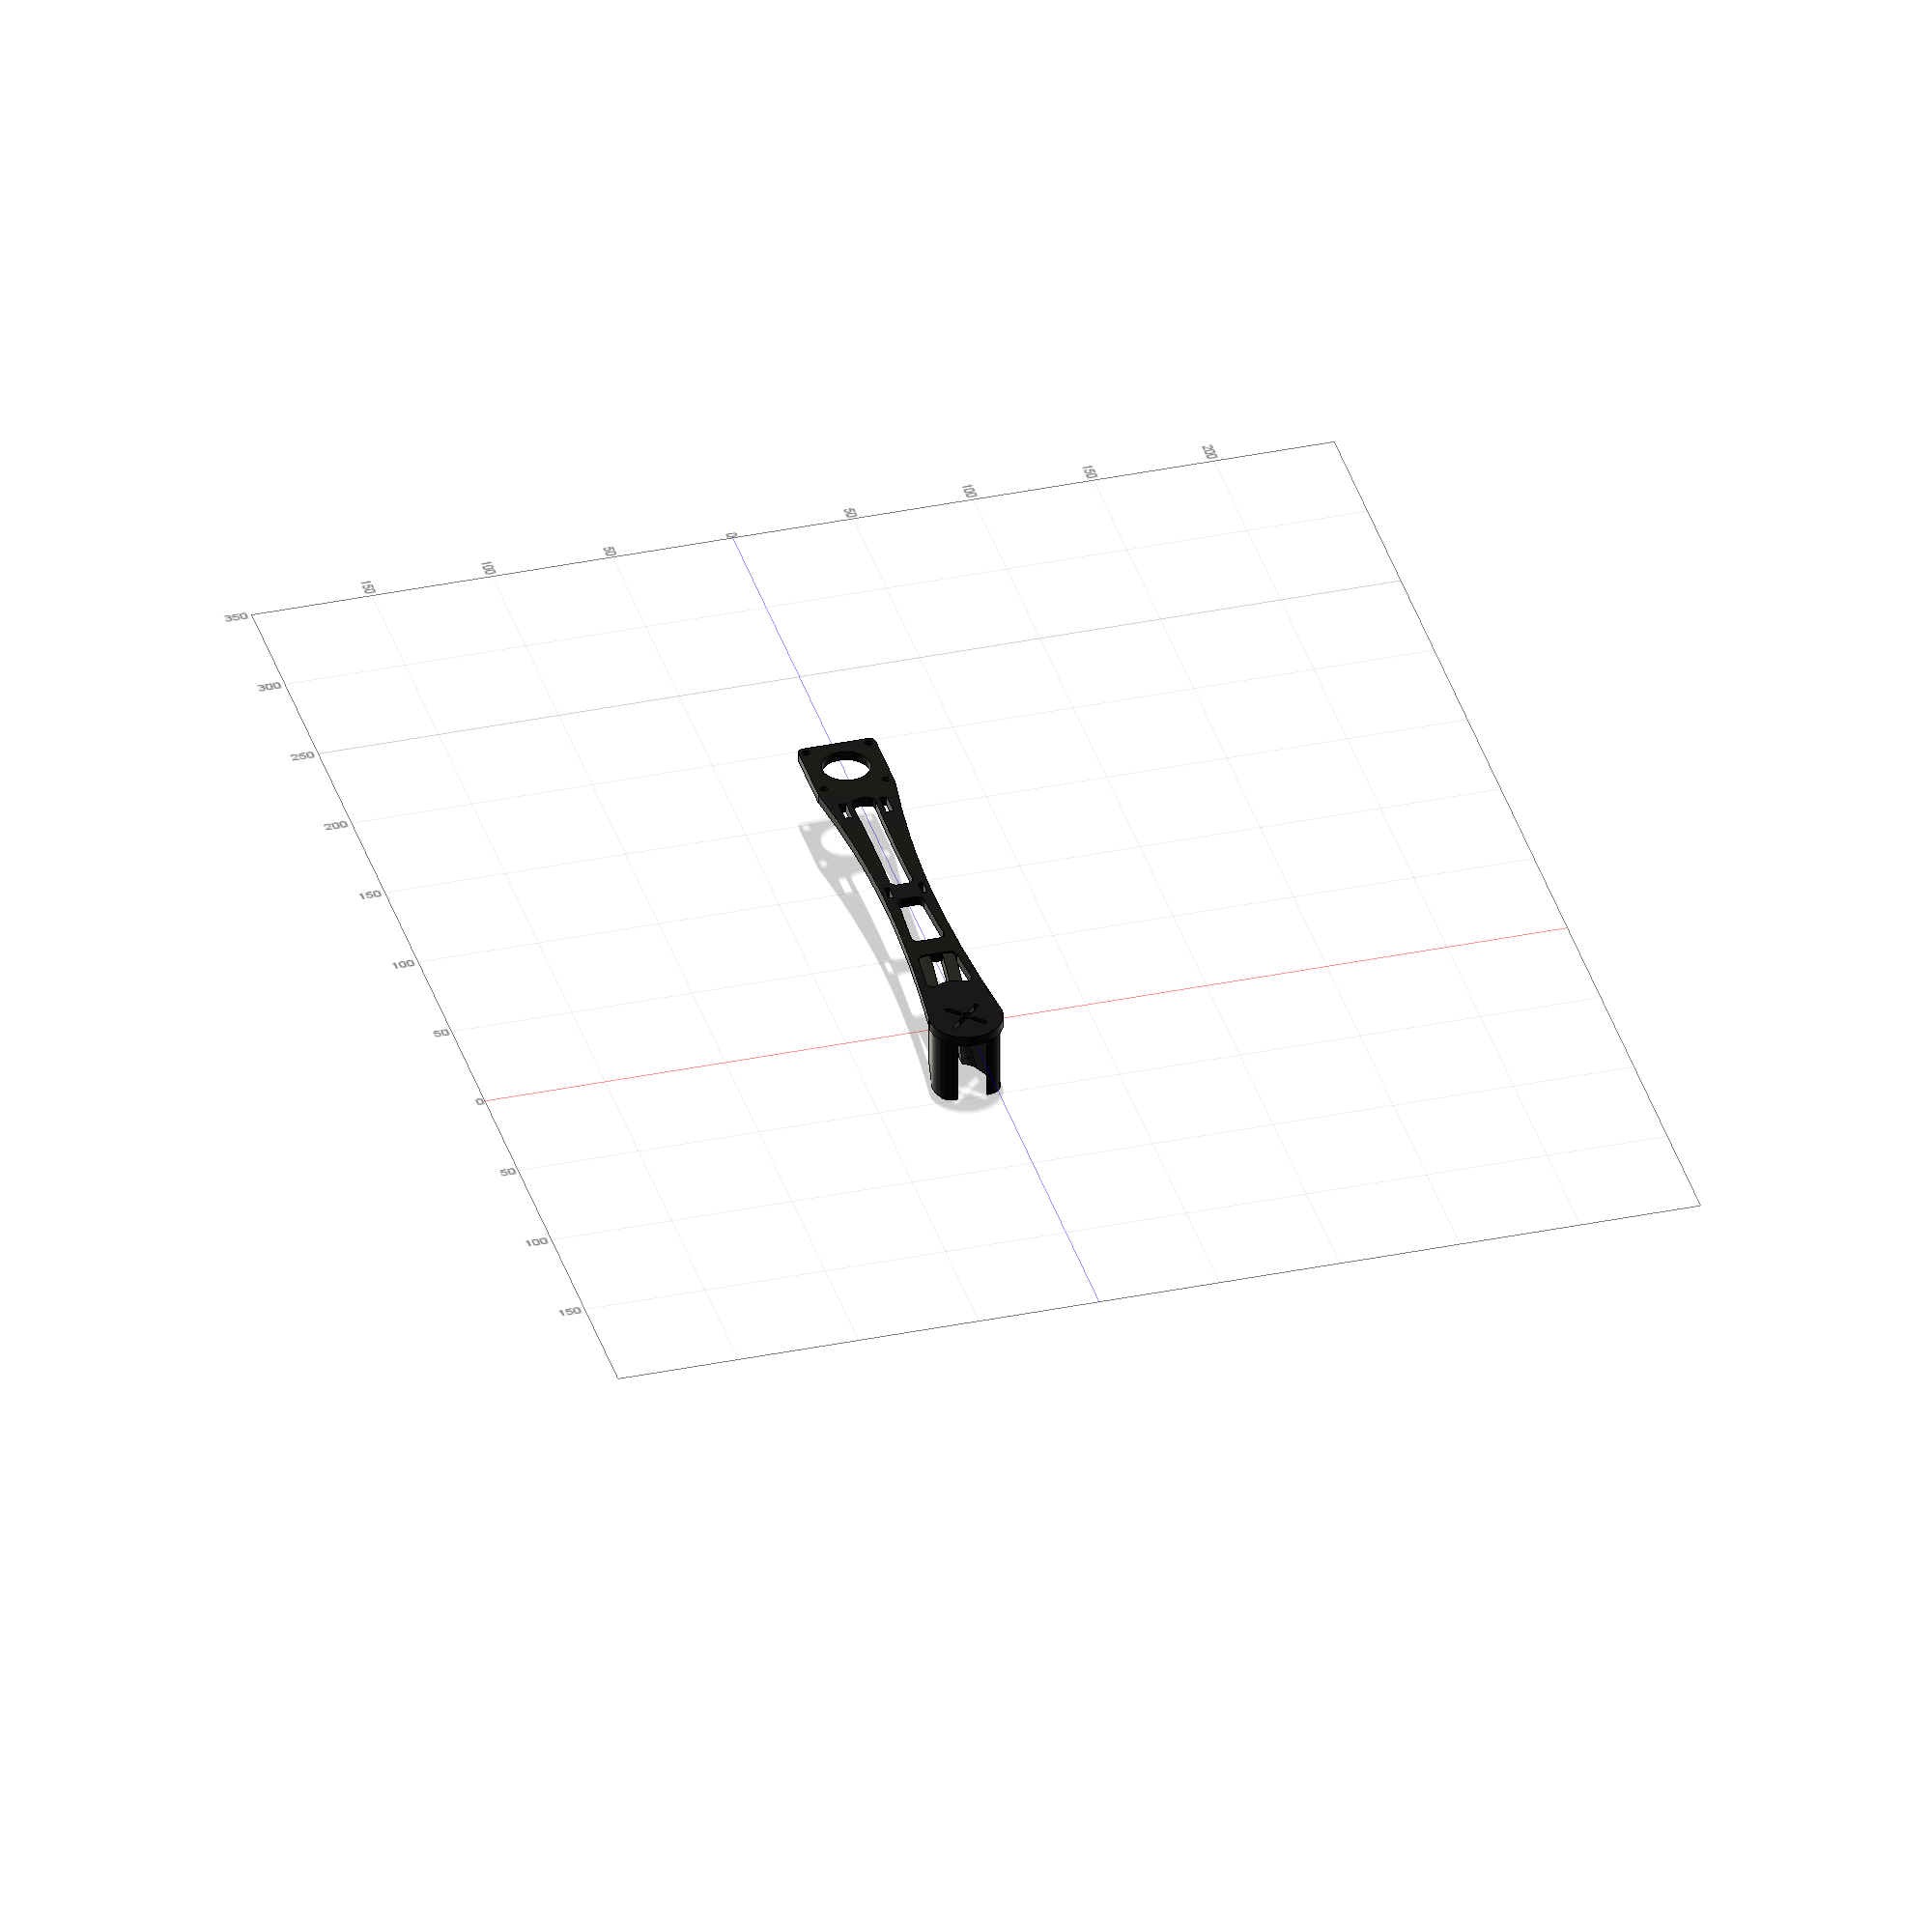
\includegraphics[width=100mm]{arm}
		\caption{Arm}
		\label{fig:arm}
	\end{figure}
	\pagebreak
	
I was really quite happy with how the arm turned out at first, however, I later realised that i would have to reinforce them with some form of stronger material in the end.
I then created a circular pattern of said arm (fig. 4) and started designing a mounting plate (fig. 5) 
\begin{figure}[h]
	\centering
	\begin{minipage}{.5\textwidth}
		\centering
		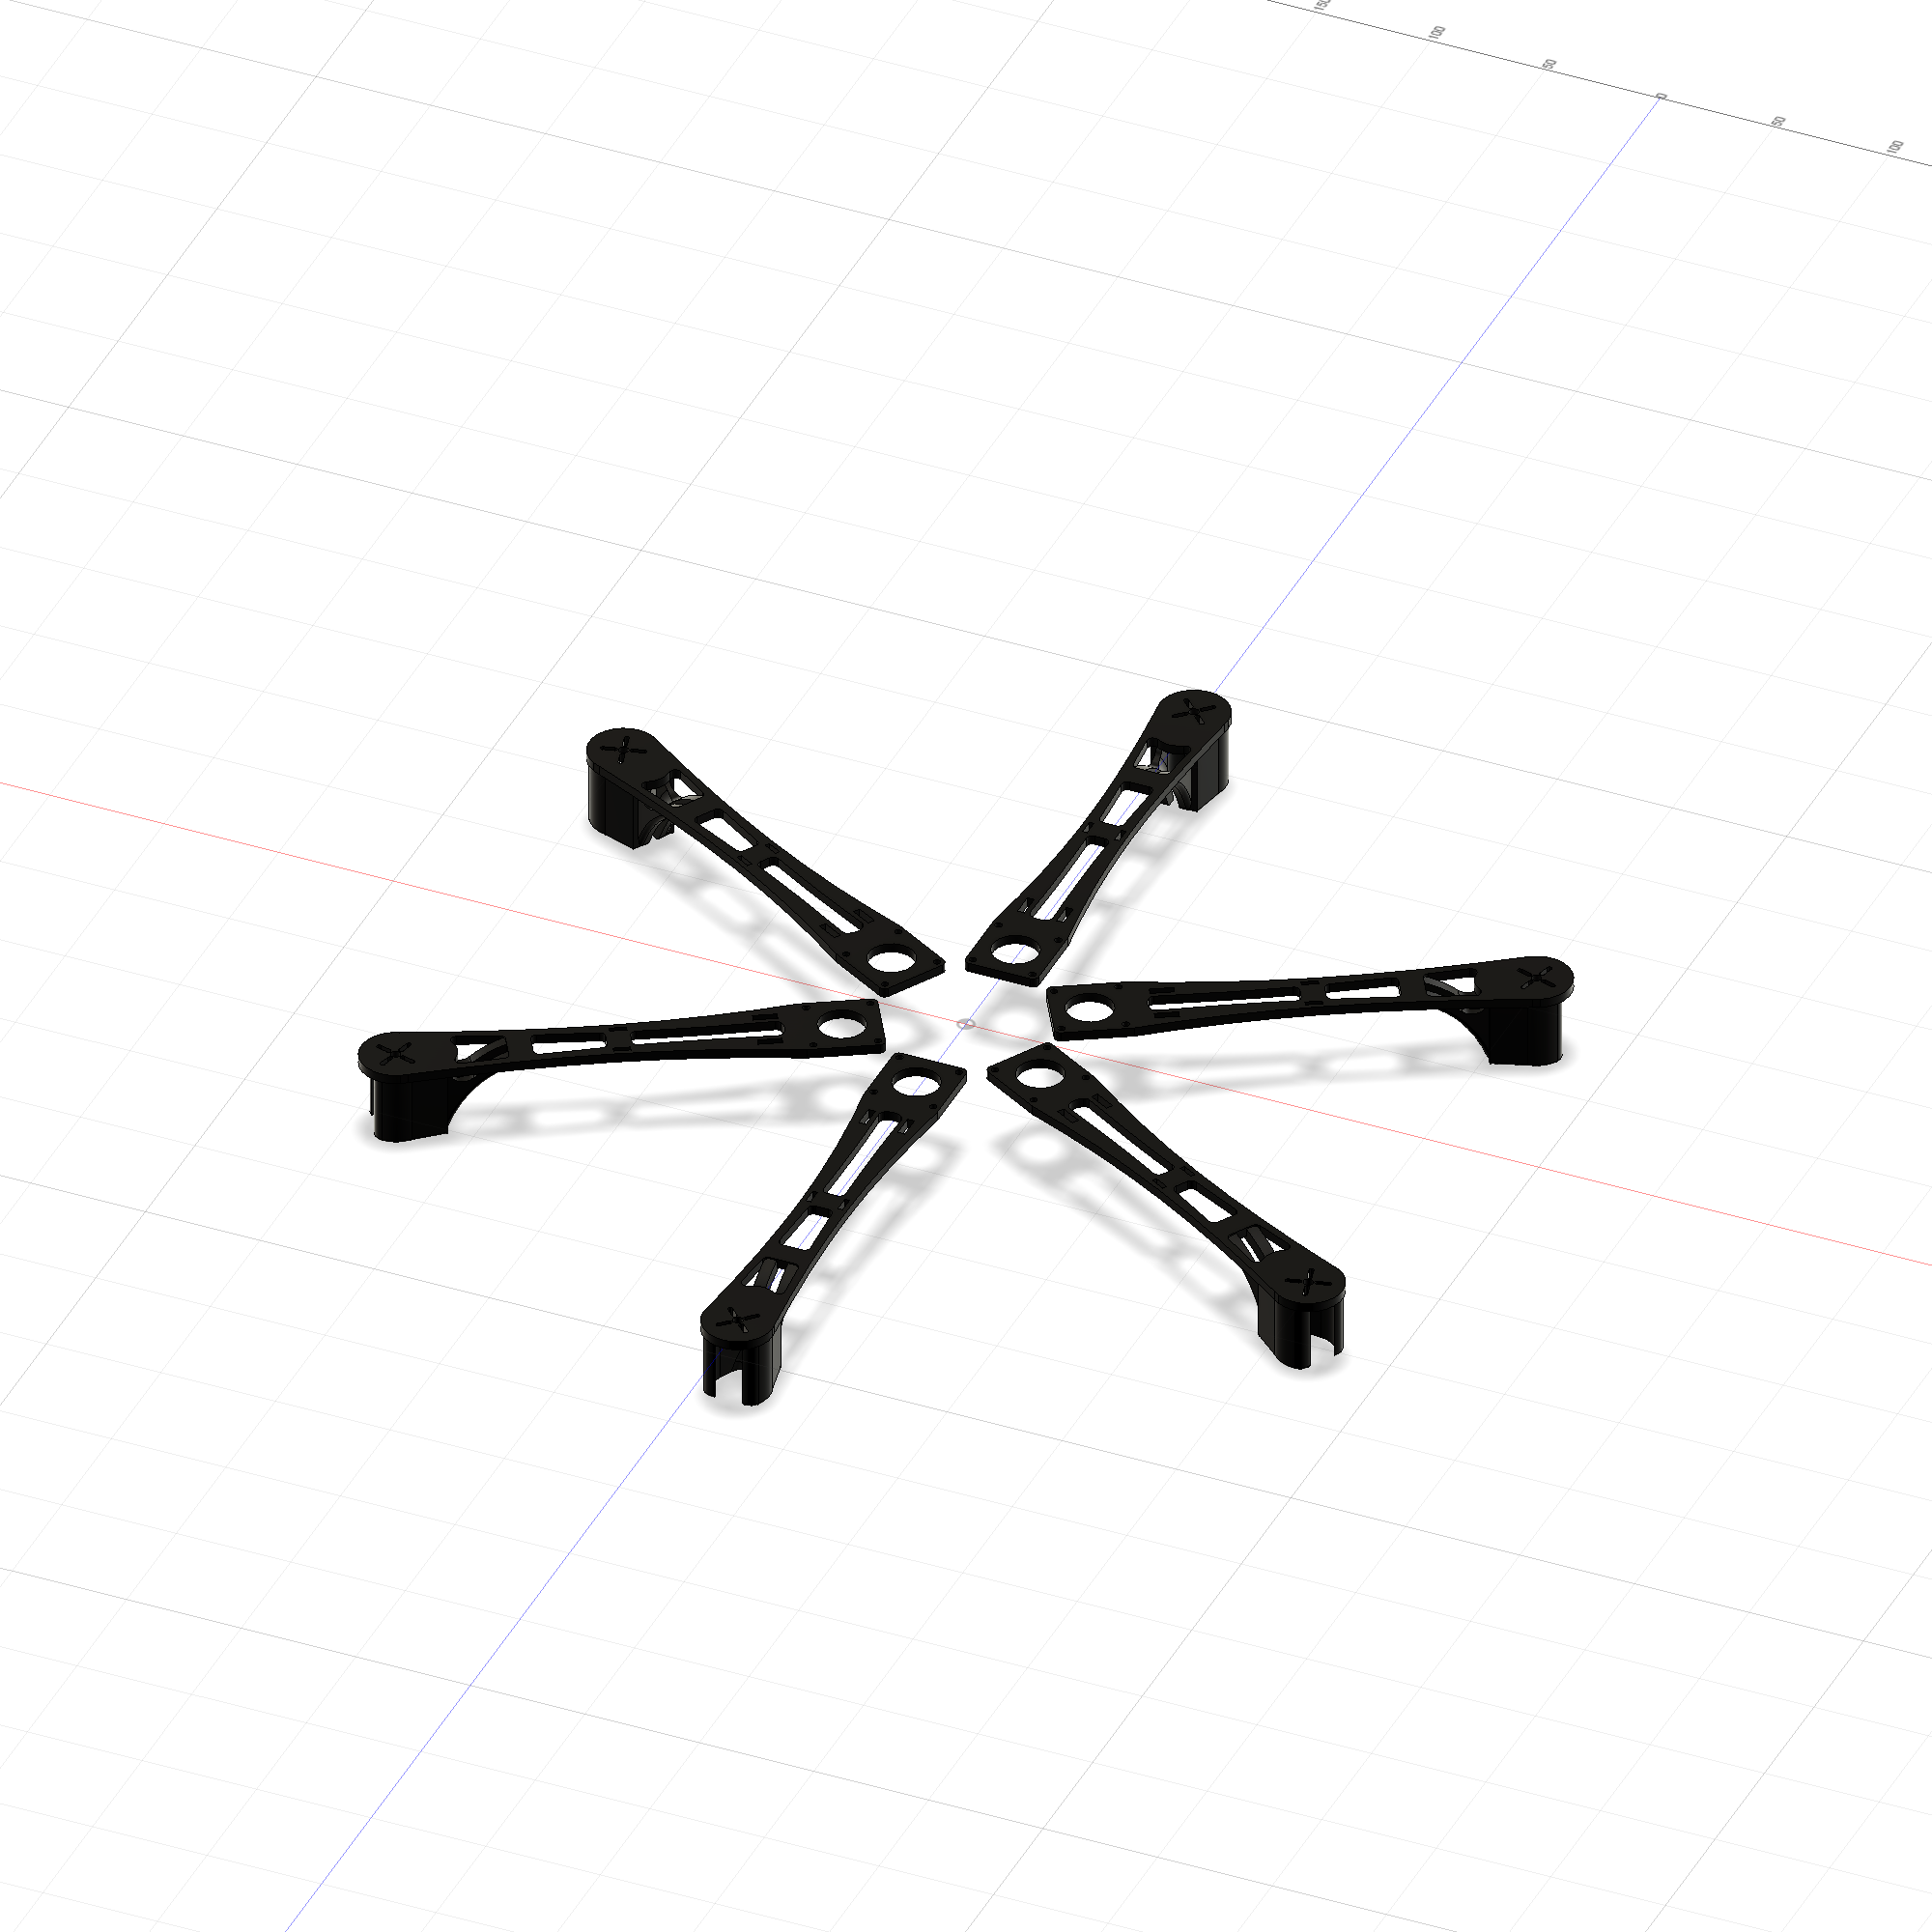
\includegraphics[width=.9\linewidth]{arms}
		\captionof{figure}{Six Arms.}
		\label{fig:arms}
	\end{minipage}%
	\begin{minipage}{.5\textwidth}
		\centering
		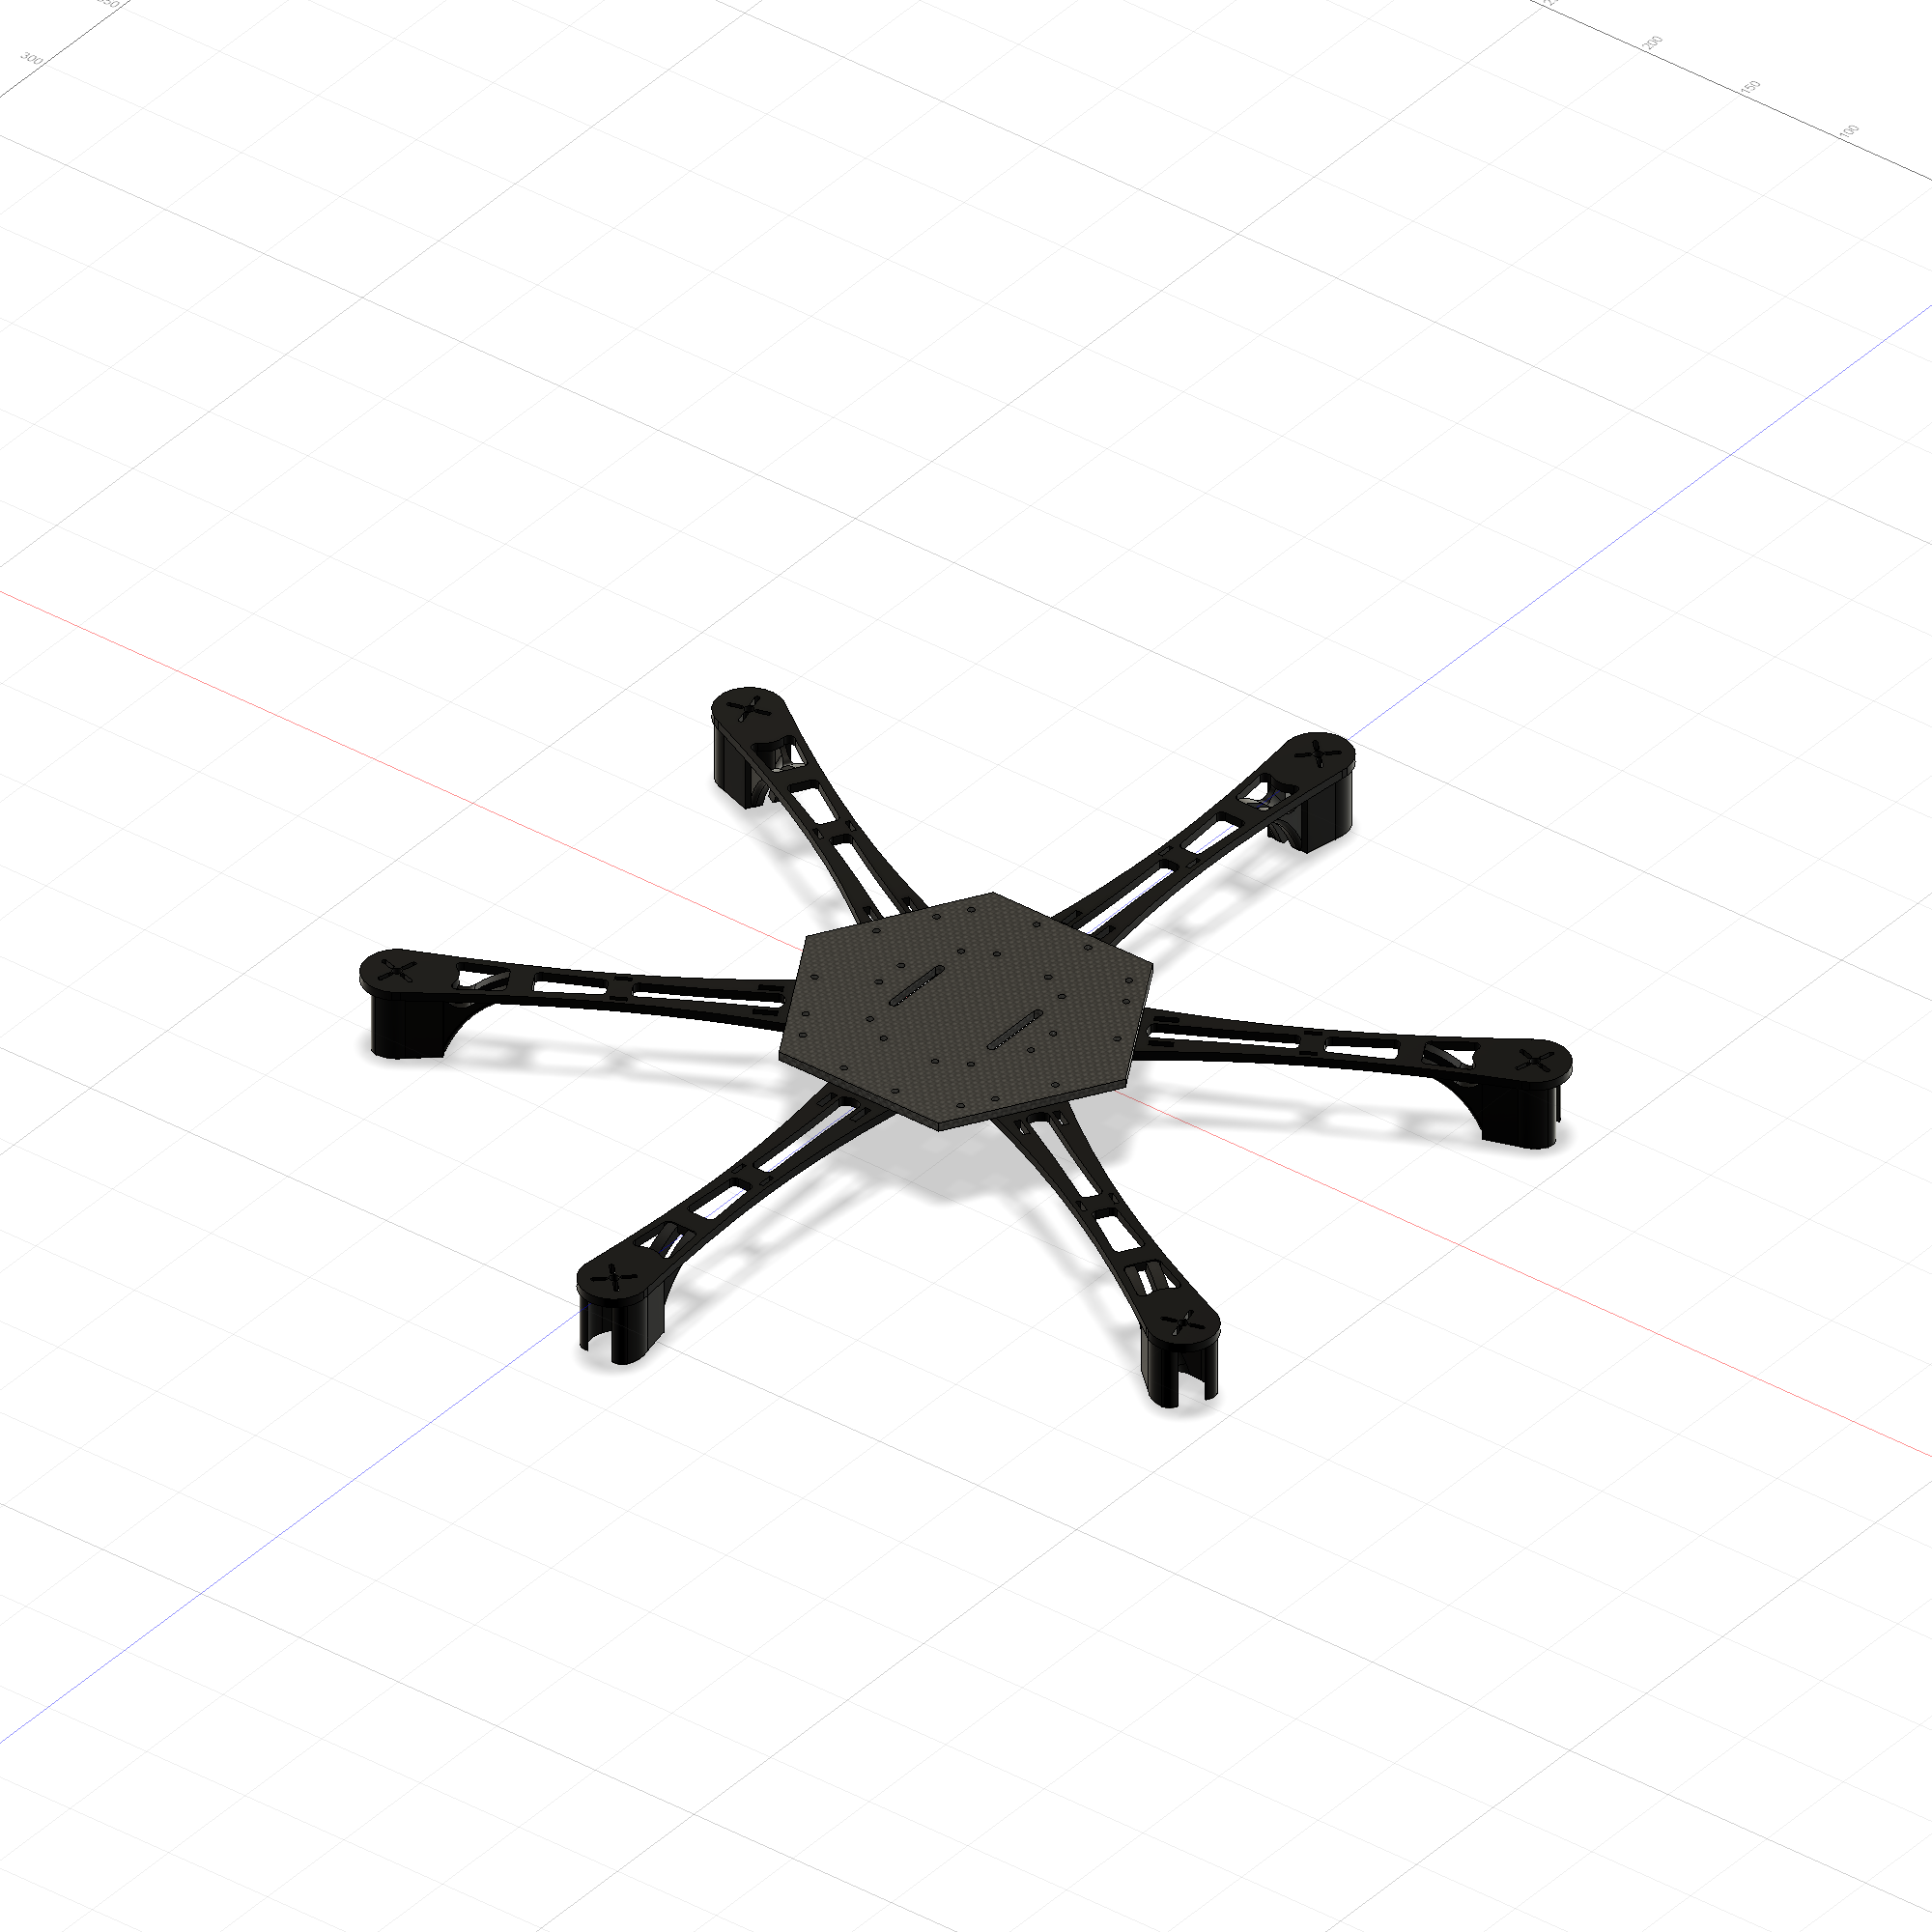
\includegraphics[width=.9\linewidth]{plate}
		\captionof{figure}{Mounting plate}
		\label{fig:plate}
	\end{minipage}
\end{figure}\newline
Then i further developed the mounting plate to support four 45mm M3 stand-offs, which would help mounting the plate for the main circuitry consisting of the Arduino and gyroscope / accelerometer. (fig. 6)\newline
I kept adding levels on top of the existing mounting plates for the GPS module and its dome. I chose to add a dome to the design as I thought it would act as protection against impact towards the fine electronics, and also because it just looks awesome. (fig. 7)
\begin{figure}[h]
	\centering
	\begin{minipage}{.5\textwidth}
		\centering
		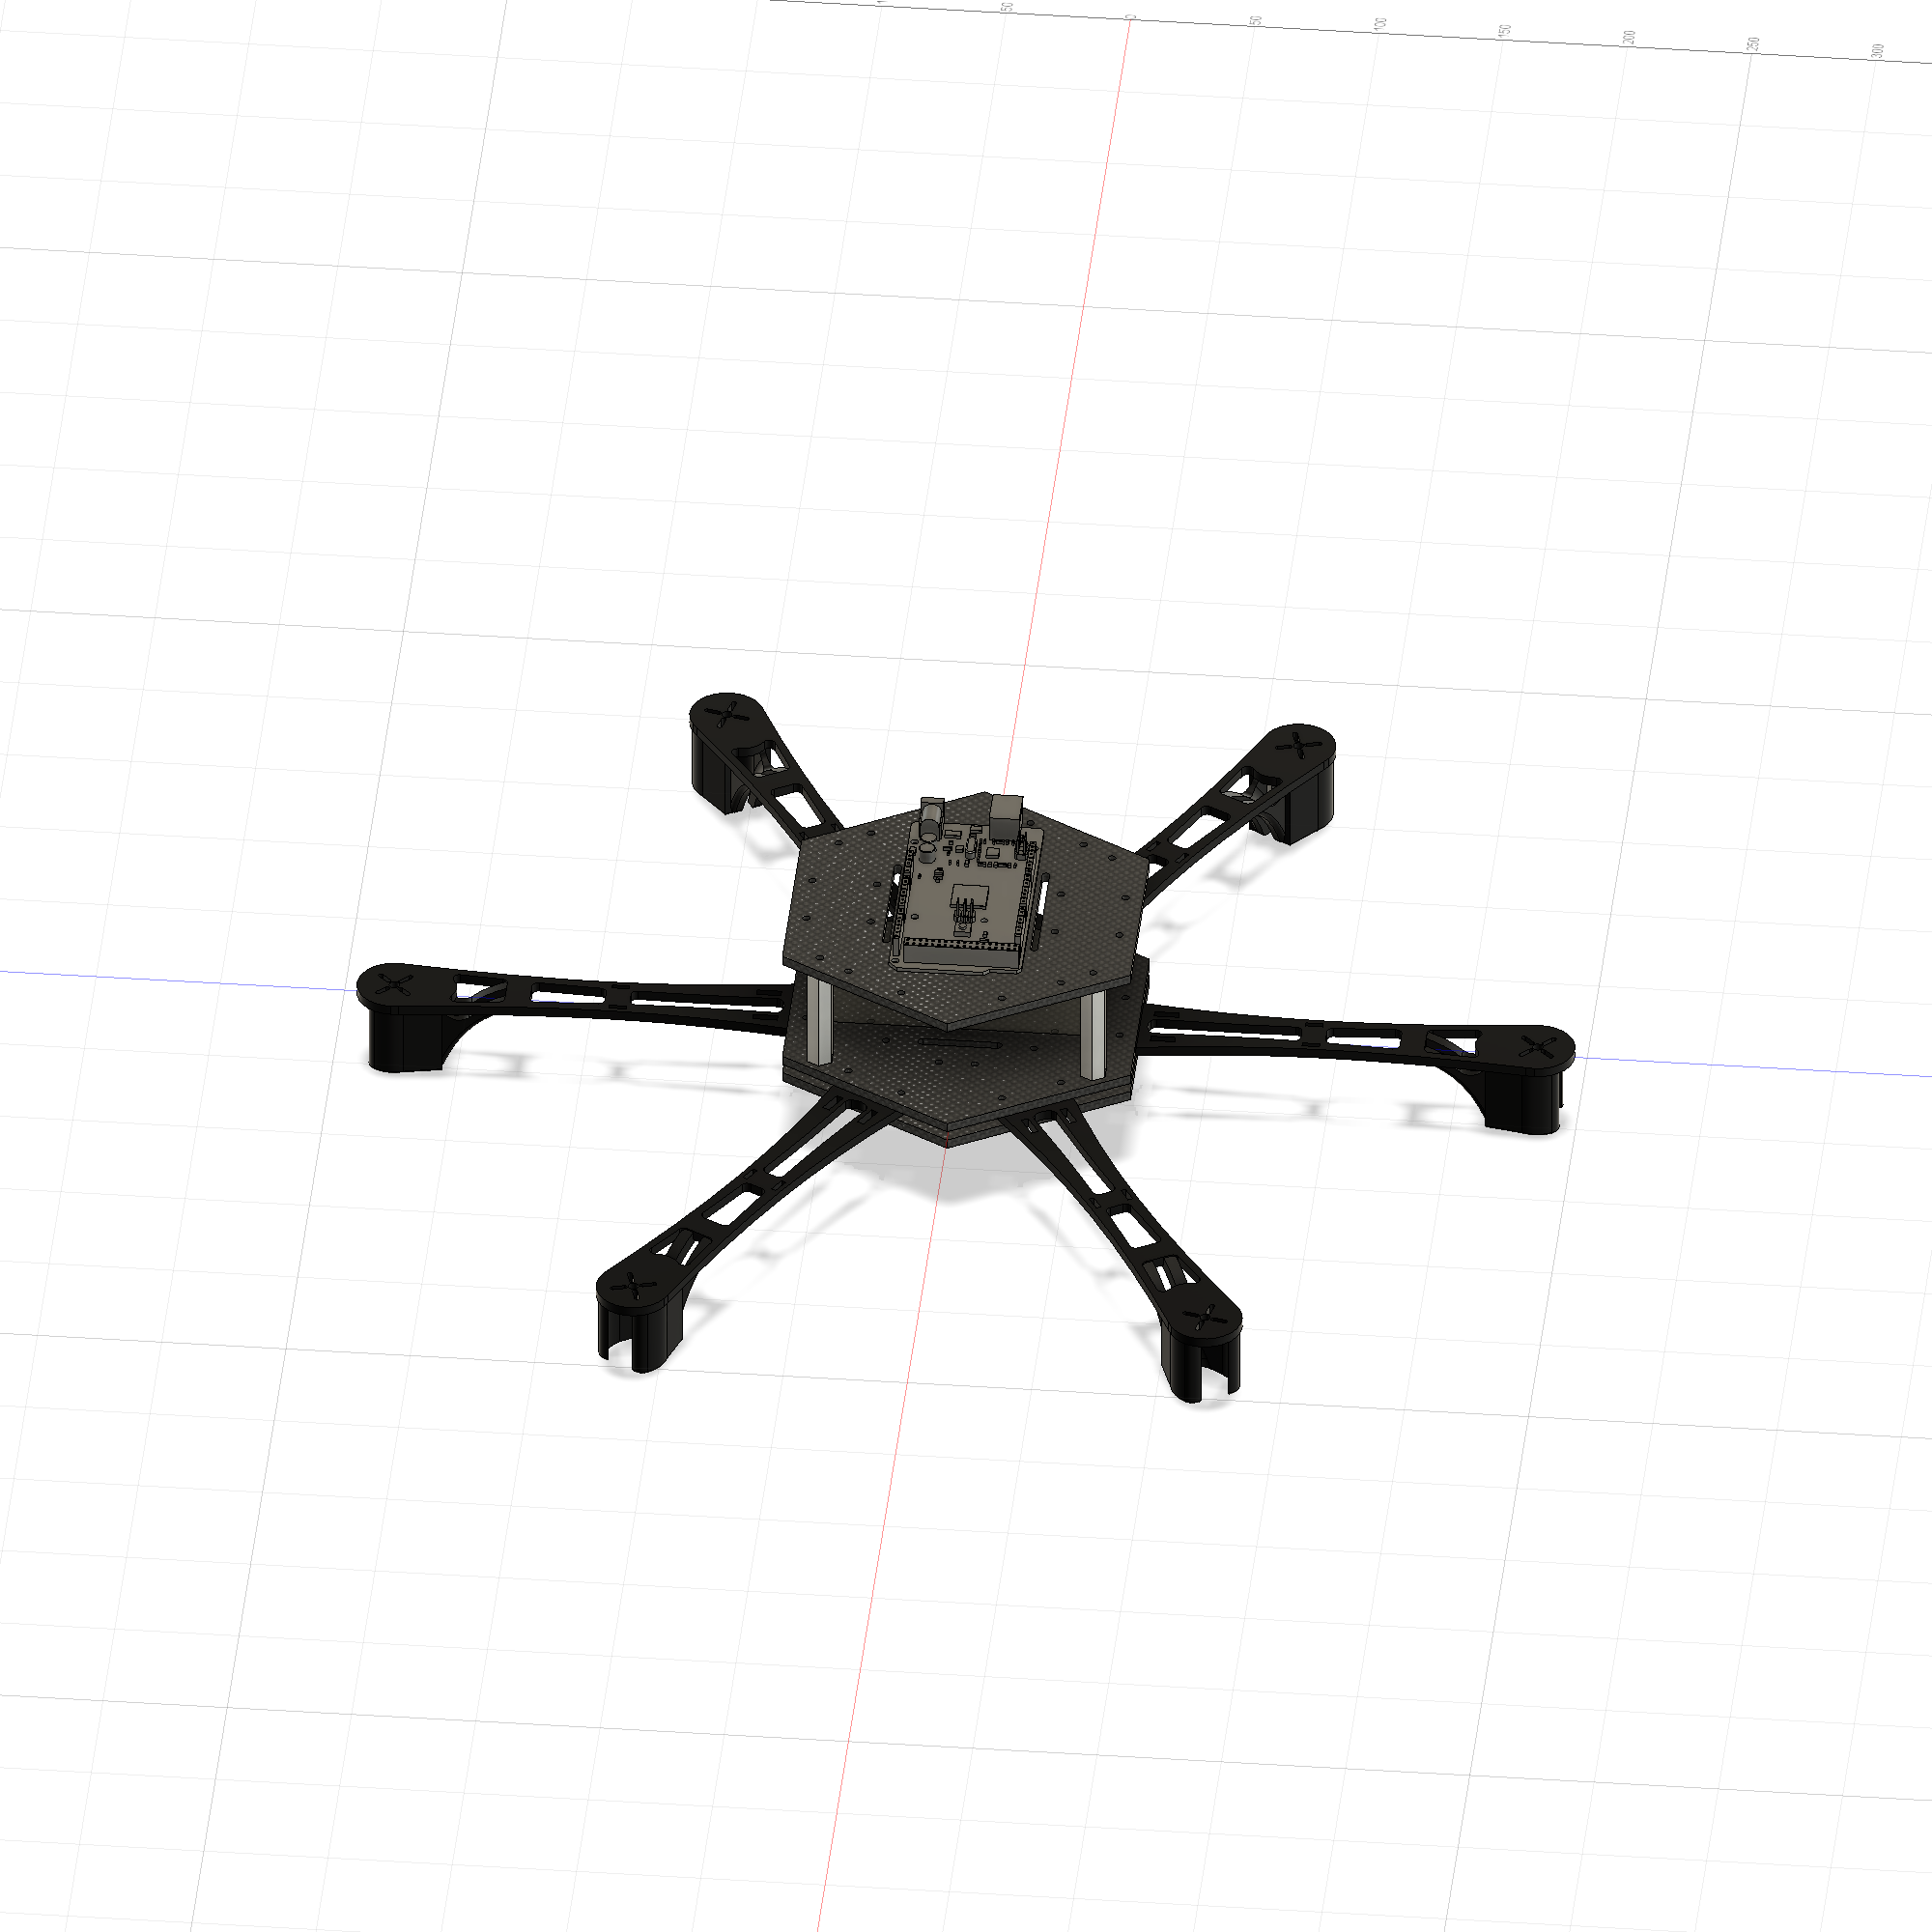
\includegraphics[width=.9\linewidth]{emount}
		\captionof{figure}{Electronics Mount}
		\label{fig:emount}
	\end{minipage}%
	\begin{minipage}{.5\textwidth}
		\centering
		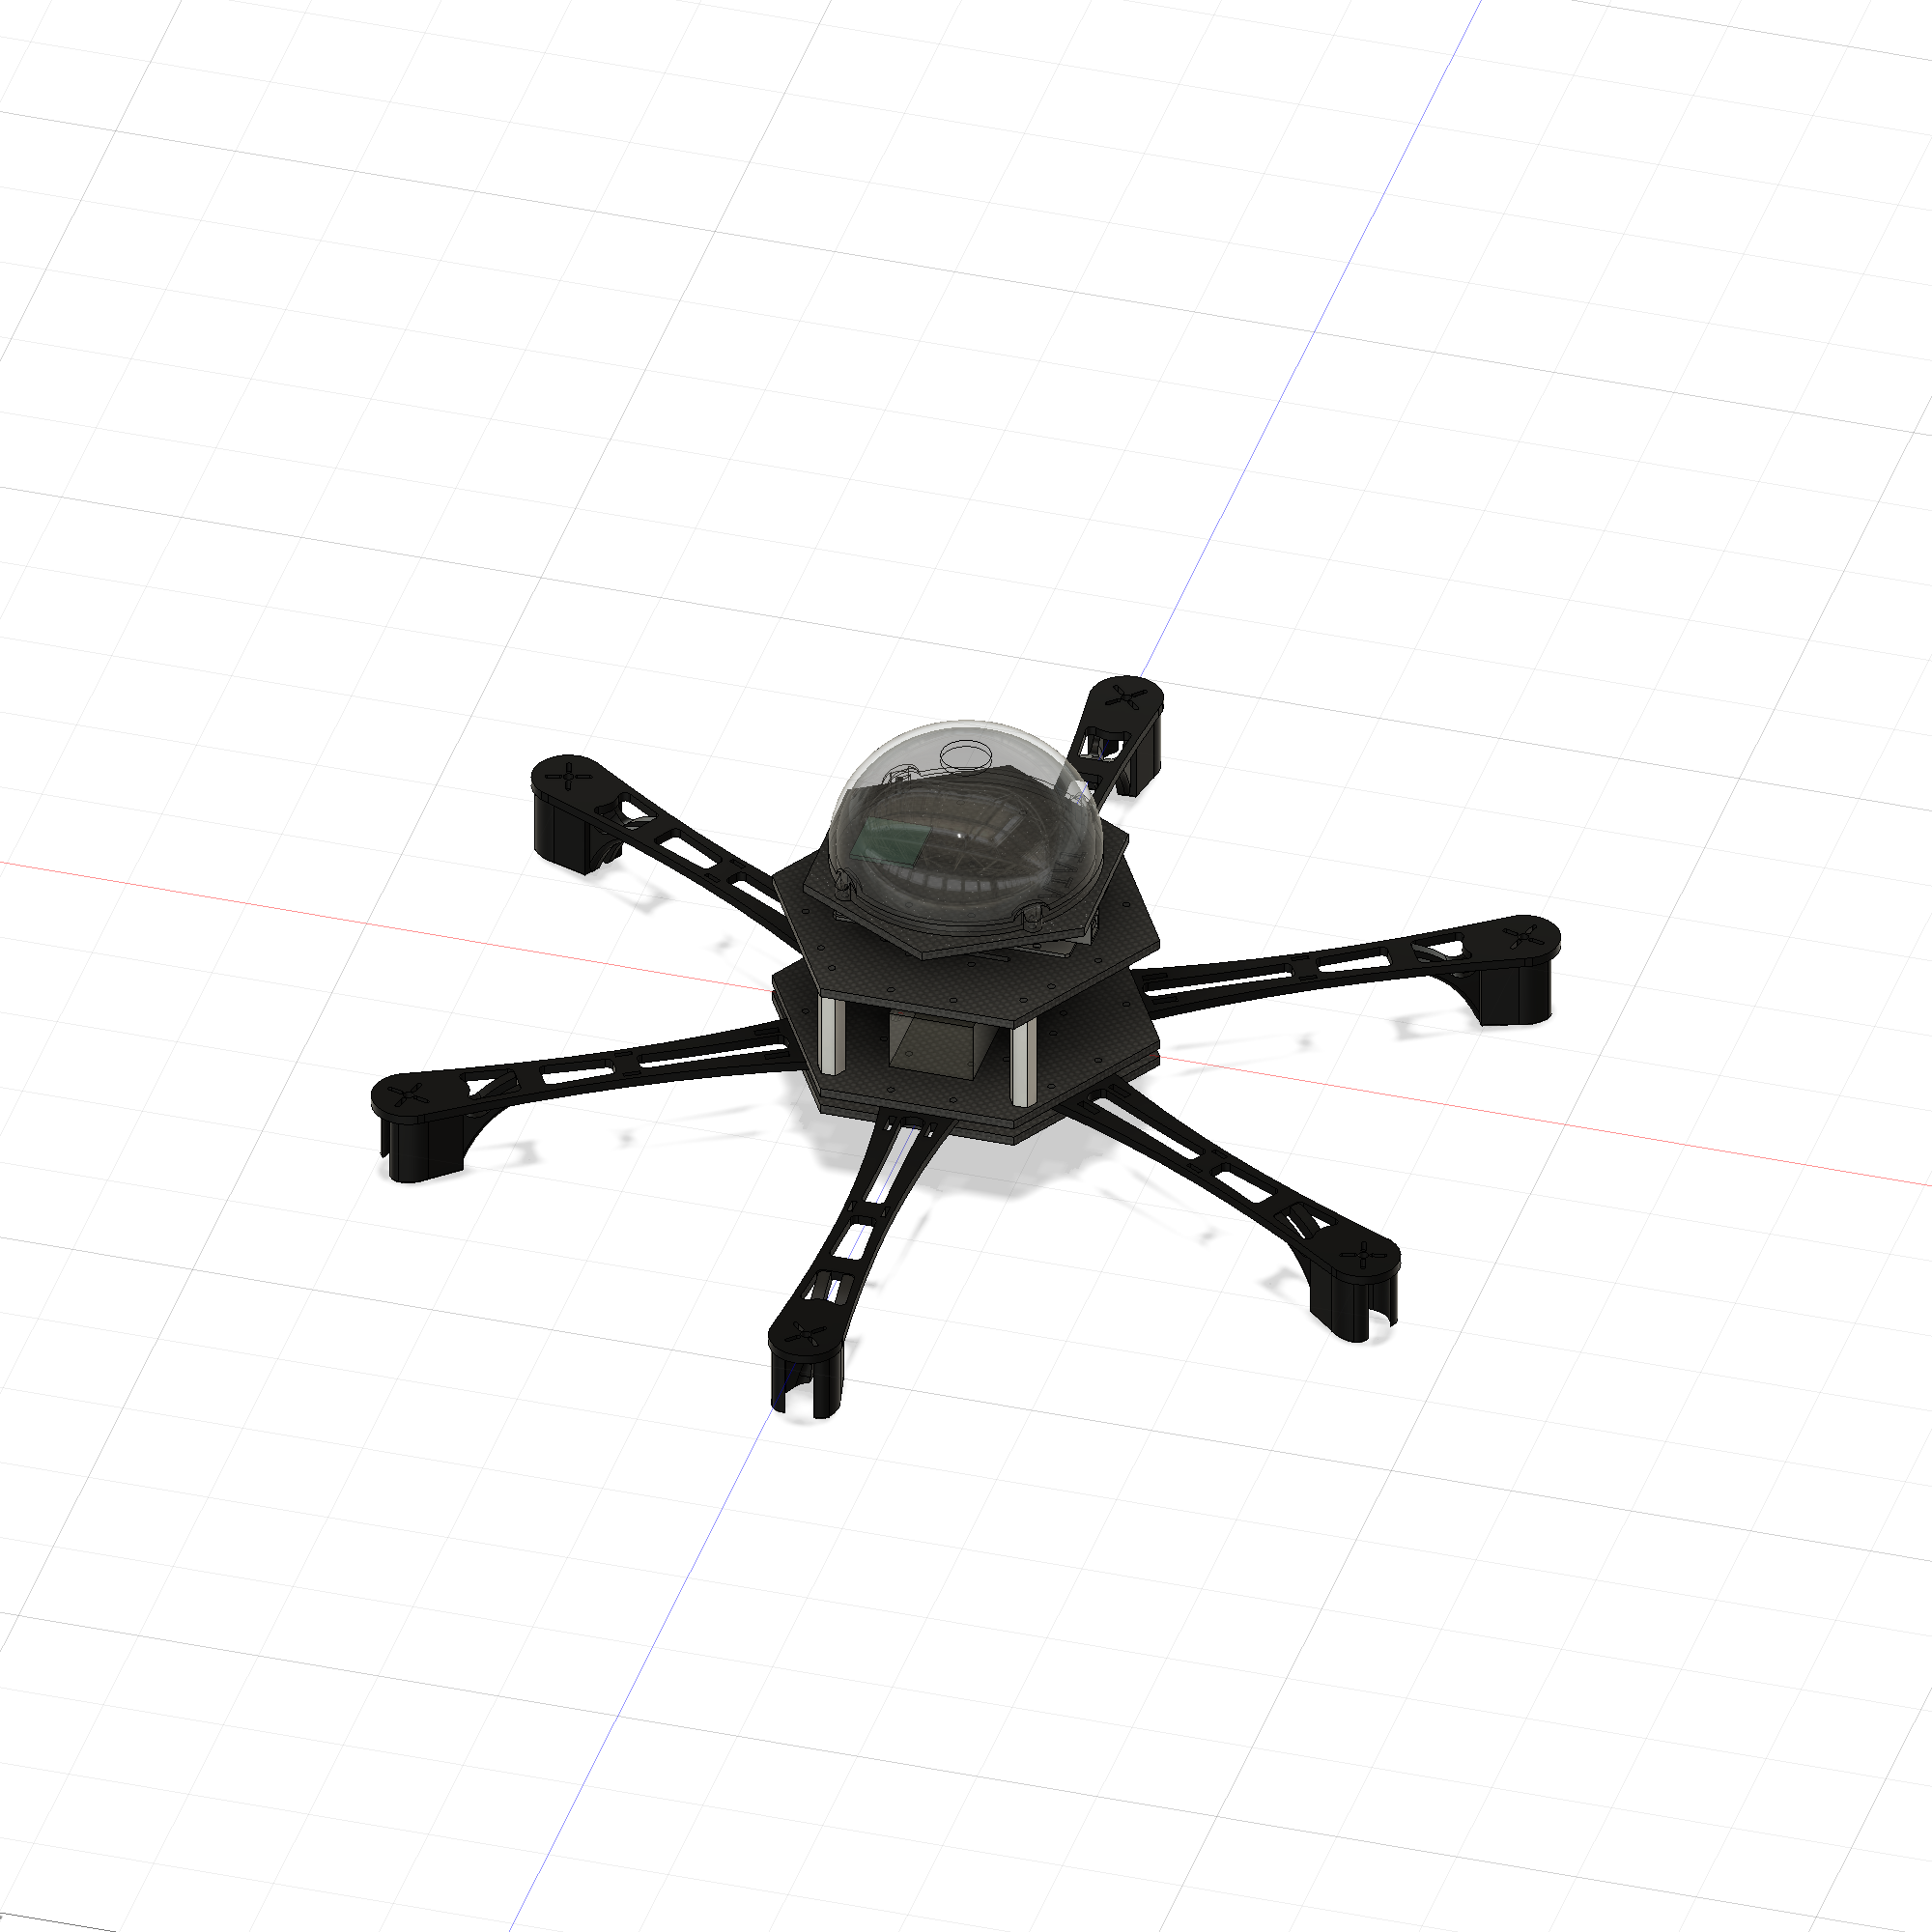
\includegraphics[width=.9\linewidth]{dome}
		\captionof{figure}{GPS and Dome}
		\label{fig:dome}
	\end{minipage}
\end{figure}
\pagebreak
At this point the design was closing up on being finished, however I still had some features that I wanted to add, namely, the ultrasonic impact protector sensors. So I created a model of a box to contain one module and positioned them where I want them to sit. I also extended the landing gear on the arms as they were not long enough to support the drone and keep the sensors from touching the ground and added modelled motors and propellers.\newline
\newline
At this point I decided to run some simulations. I started with the arms that I previously had designed, and the results were, not very good. In the Fusion 360 Simulation workspace I simulated a upwards force of 8 N (approx. 800g). The structural integrity of the arms were extremely bad and it flexed about six or seven centimetres (fig.8). This of course could not be in the finished product, so i tried making a new version that had a rib going from the landing gear to the centre of the drone (fig. 9). This part also eventually failed and only reached about one more safety point according to fusion. \newline
If I am going to be honest with you, I was sort of feeling a bit angry at this point. I had put in a lot of work on the existing arms and I did really not feel like making a completely new revision of the arm. But I did anyway. The new "3rd revision" is reinforced with a 8mm aluminium rod (hollow) (fig. 10).

\begin{figure}[h]
	\centering
	\begin{minipage}{.5\textwidth}
		\centering
		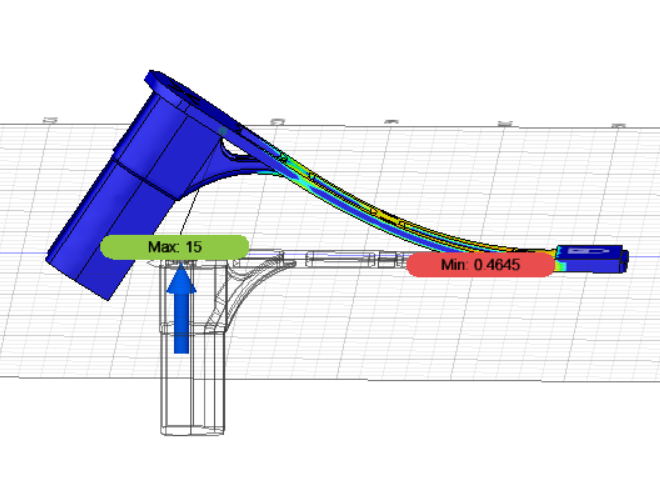
\includegraphics[width=.9\linewidth]{rev1stress}
		\captionof{figure}{Rev. 1 Stress test}
		\label{fig:r1s}
	\end{minipage}%
	\begin{minipage}{.5\textwidth}
		\centering
		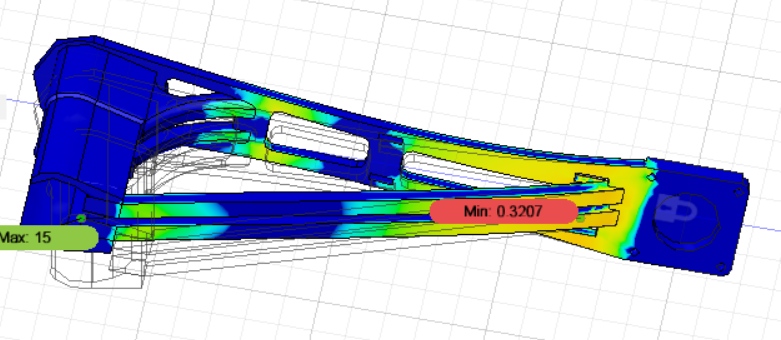
\includegraphics[width=.9\linewidth]{rev2stress}
		\captionof{figure}{Rev. 2 Stress test}
		\label{fig:r2s}
	\end{minipage}
\end{figure}
	\begin{figure}[h]
	\centering
	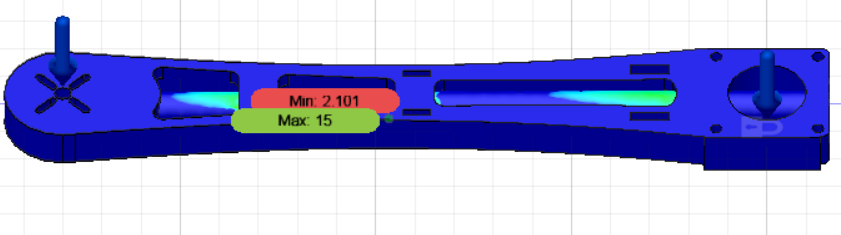
\includegraphics[width=\linewidth]{rev3stress}
	\caption{Final Stress test}
	\label{fig:r3s}
	\end{figure}

\pagebreak
	
	\subsection{Rendered image}
\begin{figure}[h]
	\centering
	\subfloat[1][Render from above]{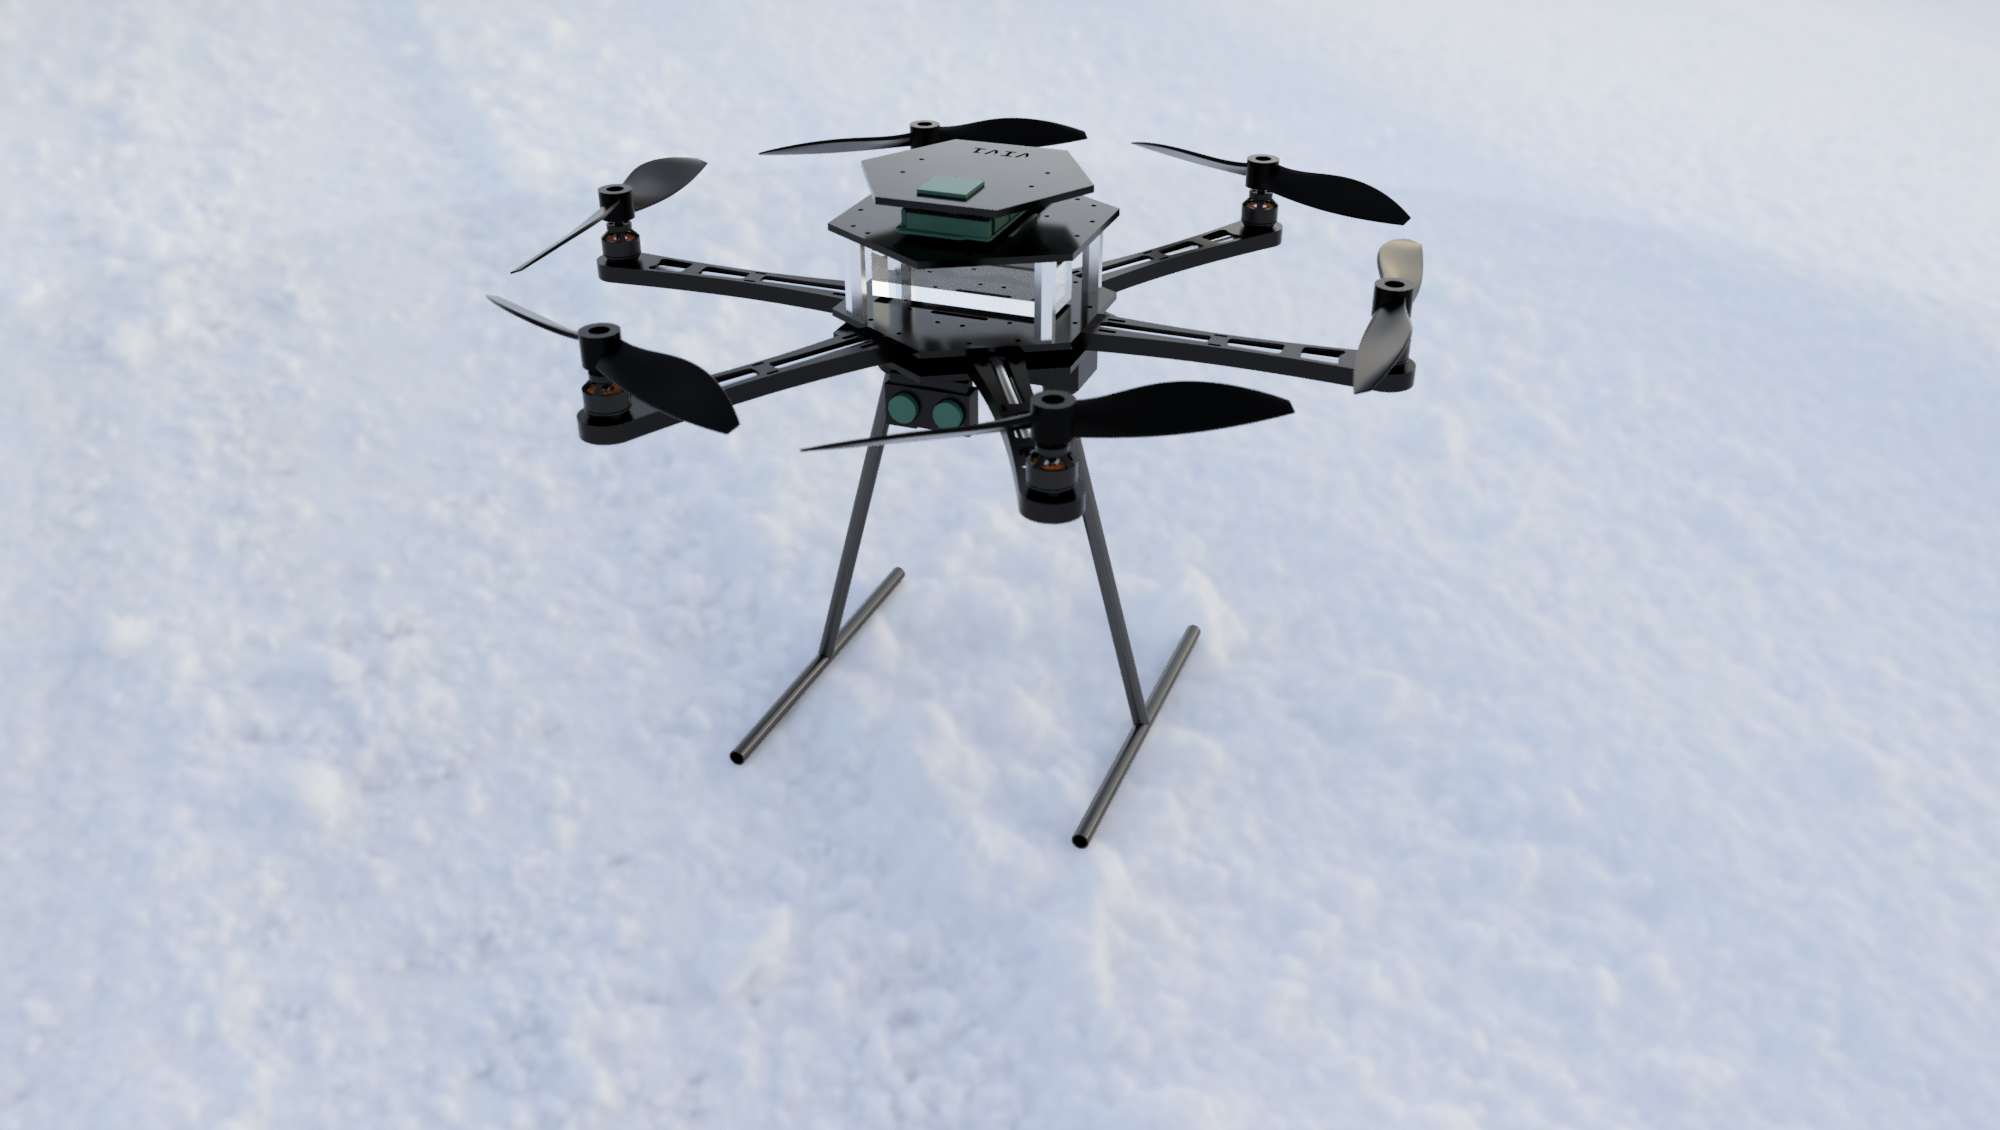
\includegraphics[width=.8\linewidth]{top.png} \label{fig:rn1}} \\
	\subfloat[2][Render from below]{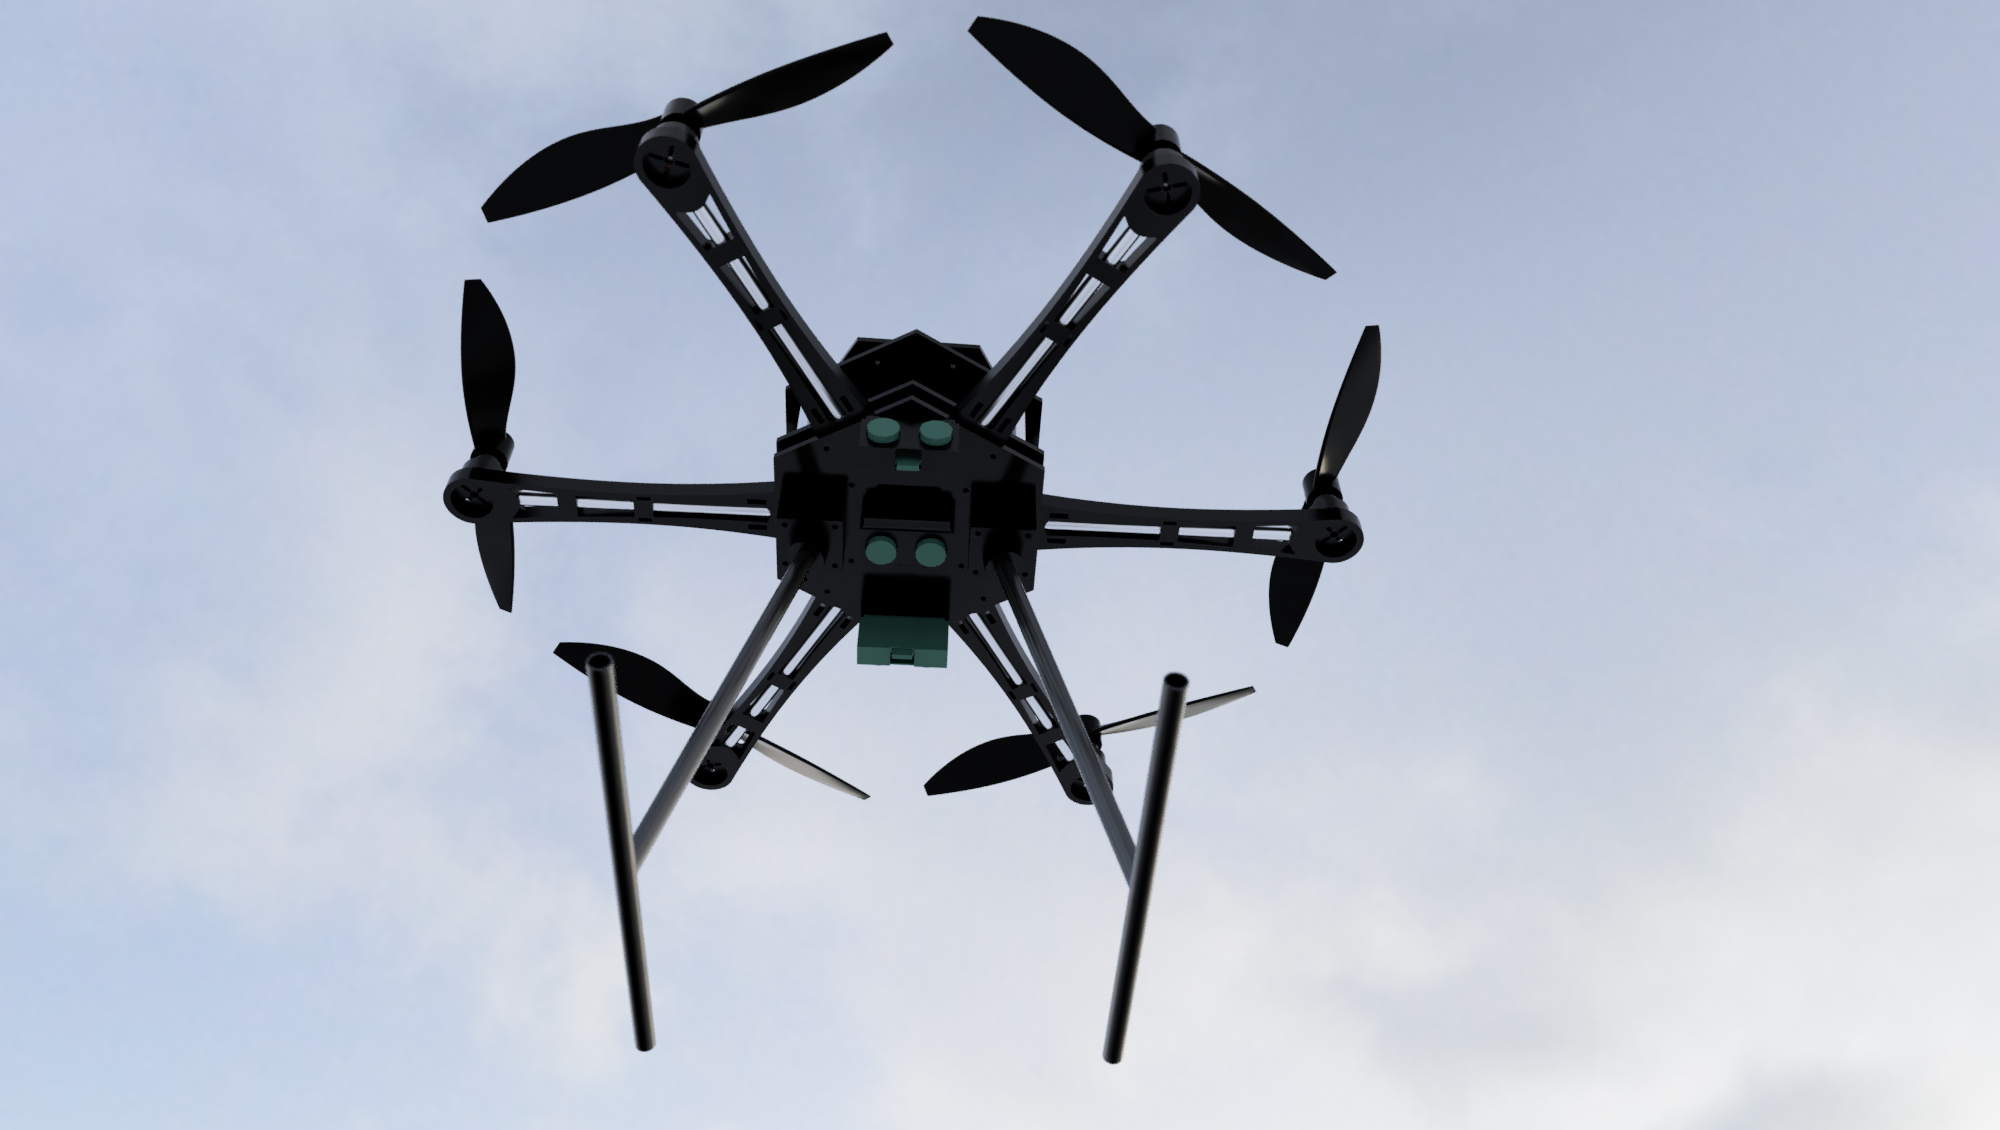
\includegraphics[width=.8\linewidth]{bottom.png} \label{fig:rn2}}
	\caption{Final Renders (note. Propeller size is off by ca 40mm.)} \label{fig:fr}
\end{figure}
\pagebreak
	\subsection{Material choice}
	The choice of materials for this product was made with weight and cost in mind. The plates are made out of Laser cut CFRP (Carbon Fibre Reinforced Plastic). The arms were 3D printed in PLA at 40 percent infill to keep the parts sturdy but also lightweight. Screws, bolts and stand-offs were made out of aluminium and stainless steel in order to keep the structure rigid at a low cost.\pagebreak
	\section{Design Process (Software)}
	\section{Construction Guide}
	\subsection{3D Printed Parts}
	\subsection{Laser Cut Parts}
	\subsection{Assembly Guide}
	\subsection{Arduino Guide}
	\subsection{Drone Firmware Documentation}
	\section{Usage}
	\section{Article License}
	
	
\end{document}
